\documentclass[conference]{IEEEtran}
\IEEEoverridecommandlockouts

\usepackage{cite}
\usepackage{amsmath,amssymb,amsfonts}
\usepackage{graphicx}
\usepackage{booktabs}
\usepackage{array}
\usepackage{multirow}
\usepackage{xcolor}
\usepackage{url}
\usepackage{pgfplots}
\pgfplotsset{compat=1.17}
\usepackage[hidelinks]{hyperref}

\definecolor{cA}{HTML}{1F77B4}
\definecolor{cB}{HTML}{D95F02}
\definecolor{cC}{HTML}{2CA02C}
\definecolor{cD}{HTML}{7B3FA0}

\newcommand{\cm}{\checkmark}
\newcommand{\best}[1]{\textbf{#1}}

\begin{document}

\title{Adaptive Hybrid Semantic Research Assistant:\\
Retrieval-First, Evidence-Grounded Extractive Question Answering}

\author{\IEEEauthorblockN{A. R. Nirmal, Gunnala Dheeraj Kumar, Meera S Raj, and Vishnu Vardhan N}
\IEEEauthorblockA{23AID472 Text Analytics, Batch A-17}}

\maketitle

\begin{abstract}
Keyword search misses paraphrases, dense semantic search misses exact terms, and generative
language models can produce fluent answers that no source supports. This paper presents the
Adaptive Hybrid Semantic Research Assistant, a retrieval-first question answering system in
which every answer is a span copied from a retrieved passage. The system fuses BM25 and
Sentence-BERT retrieval with Reciprocal Rank Fusion, expands each question into rule-based
variants, re-ranks candidates with a cross-encoder, and extracts the answer with a fine-tuned
transformer reader. On SQuAD v1.1 the retrieval stack raises Recall@10 from 86.15\% for BM25 to
96.25\% and Mean Reciprocal Rank from 69.49\% to 85.25\%, removing 73\% of first-stage retrieval
misses. The RoBERTa-base reader reaches 85.38 Exact Match and 91.74 F1 on the full
10,570-question development set, which exceeds human performance, the published BERT-base and
DistilBERT results, and the published single-model BERT-large result, and is within 0.1 F1 of the
BERT-large ensemble. End to end, the system answers 71.0\% of questions exactly. The whole stack
uses open models, runs on one 8~GB laptop GPU, and returns evidence, confidence and latency with
every answer.
\end{abstract}

\begin{IEEEkeywords}
question answering, hybrid retrieval, reciprocal rank fusion, cross-encoder re-ranking,
extractive reading comprehension, SQuAD, RoBERTa
\end{IEEEkeywords}

%% ---------------------------------------------------------------------------
\section{Introduction}

Open-domain textual question answering (QA) answers a question from a large collection instead of
from one supplied paragraph. Progress in the task is driven by two developments, machine reading
comprehension and neural information retrieval, which together let a system retrieve relevant
text and read it to extract an answer \cite{huang2020}. The retrieval side is commonly organised
in two stages: a fast first stage selects candidates from the whole collection, and a slower,
stronger second stage re-scores them \cite{hambarde2023}.

Each building block has a known weakness. Lexical ranking with BM25 \cite{robertson2009} rewards
exact matches of distinctive terms but gives no credit to a passage that answers the question in
different words. Dense retrieval with sentence embeddings \cite{reimers2019} matches meaning but
can under-weight rare names and identifiers. Generative answering reads well, yet unfaithful
output is a major risk wherever language models would otherwise be useful \cite{malin2025}.

This paper describes a system that combines the complementary strengths and removes the
faithfulness risk by construction. It retrieves with both BM25 and a bi-encoder, fuses the
rankings by position, re-ranks the fused candidates with a cross-encoder, and extracts the answer
as a span of the top passage. An answer therefore cannot contain text that is absent from the
evidence shown to the user.

The contributions are:
\begin{itemize}
\item a complete hybrid retrieval and extractive QA pipeline built only from open models that
      run locally on a single 8~GB laptop GPU;
\item a lightweight adaptive query layer, with rule-based complexity estimation that sets the
      retrieval depth and multi-query expansion that needs no additional model;
\item a seven-configuration ablation that measures the contribution of every retrieval stage
      with standard ranking metrics on a public benchmark;
\item a dual-setting evaluation of three readers, with the gold passage and end to end behind
      the same retriever, which locates the remaining error in the pipeline;
\item results that match or exceed published reference points: 96.25\% Recall@10 for retrieval
      and 85.38 EM / 91.74 F1 for reading on SQuAD v1.1.
\end{itemize}

%% ---------------------------------------------------------------------------
\section{Related Work}

\subsection{Sparse and Passage-Level Retrieval}
BM25 scores a passage by summing, over the query terms, an inverse-document-frequency weight
multiplied by a saturating term-frequency component with length normalisation
\cite{robertson2009}. It needs no training data. Dang \emph{et al.} \cite{dang2021} showed on
several TREC collections that scoring documents through their passages performs significantly
better than scoring whole documents, which supports indexing at a finer granularity than full
articles.

\subsection{Dense Retrieval and Vector Search}
Text representation has moved from rule-based and statistical methods to contextual learned
embeddings \cite{patil2023}. Sentence-BERT encodes each sentence independently into a fixed
vector, reducing the search for the most similar pair among 10,000 sentences from about 65 hours
with BERT to about 5 seconds \cite{reimers2019}. Dual encoders are now widely used for
open-domain QA: Dense Passage Retrieval trains them with in-batch negatives
\cite{karpukhin2020}, and adaptive batch scheduling makes those negatives progressively harder
\cite{choi2021}. Tan \emph{et al.} \cite{tan2025} observe that embedding a long text into one
vector loses information, a direct motivation for chunking. FAISS provides exact and approximate
nearest-neighbour search at billion scale \cite{johnson2021}.

\subsection{Hybrid Retrieval, Fusion and Query Expansion}
BM25 scores and cosine similarities lie on unrelated scales. Reciprocal Rank Fusion (RRF) avoids
calibration by combining rankings by position, and outperformed Condorcet fusion and individual
learning-to-rank methods \cite{cormack2009}. Recent IEEE work confirms the value of hybrids:
Bindle \emph{et al.} \cite{bindle2025} combine TF-IDF and BM25 with Sentence-BERT and Word2Vec
using query-adaptive weights, and Khan \emph{et al.} \cite{khan2026} fuse BM25 with dense
embeddings through RRF inside a retrieval-augmented generation system. Query expansion addresses
the mismatch between one phrasing of a question and the wording of the answering passage; Raza
\emph{et al.} \cite{raza2019} organise semantic expansion methods into a taxonomy, and Mageshwari
and Shrijith \cite{mageshwari2026} combine language-model expansion with RRF.

\subsection{Neural Re-ranking}
Keyword features cannot capture contextual relationships between query and passage, whereas
BERT-based rankers capture them far better at the cost of labelled training data
\cite{kim2022}. Kim and Ko obtained the best non-ensemble MRR@10 on the MS~MARCO passage
re-ranking leaderboard with multitask fine-tuning \cite{kim2022}.

\subsection{Extractive Reading Comprehension}
SQuAD contains over 100,000 crowd-sourced questions whose answers are spans of Wikipedia
paragraphs \cite{rajpurkar2016}. BERT introduced deep bidirectional pre-training followed by
fine-tuning \cite{devlin2019}; RoBERTa showed that BERT was under-trained and improved the
pre-training recipe \cite{liu2019}; DistilBERT is 40\% smaller and 60\% faster while retaining
97\% of BERT's language-understanding capability \cite{sanh2019}. Liu \emph{et al.}
\cite{liu2023} note that retrieve-then-extract pipelines suffer from error propagation.
Sinthusha \emph{et al.} \cite{sinthusha2025} compare transformer readers on a translated SQuAD,
and Huang \emph{et al.} \cite{huang2023} show that distillation retains over 95\% of BERT's
accuracy with about half the parameters.

\subsection{Grounding and Faithfulness}
Hypothetical Prompt Embeddings improve chunk-level retrieval for grounded answers
\cite{vake2025}, and Malin \emph{et al.} \cite{malin2025} review how faithfulness is measured
across summarisation, QA and translation.

\subsection{Positioning}
Table~\ref{tab:position} places this work against the six most closely related IEEE
publications. Earlier systems tend to report end results with generation-oriented metrics or to
depend on proprietary or per-query language models. This work keeps the same proven building
blocks, runs them with open models only, and reports the contribution of every stage with
ranking metrics.

\begin{table*}[t]
\centering
\caption{Positioning against the most closely related IEEE publications}
\label{tab:position}
\footnotesize
\renewcommand{\arraystretch}{1.15}
\begin{tabular}{@{}p{0.11\textwidth}p{0.2\textwidth}p{0.19\textwidth}p{0.19\textwidth}p{0.2\textwidth}@{}}
\toprule
\textbf{Work} & \textbf{Approach} & \textbf{Limitation} & \textbf{This work} & \textbf{Our evidence} \\
\midrule
Khan \emph{et al.} \cite{khan2026} &
BM25 + OpenAI embeddings fused with RRF; answers generated by an LLM (BERTScore F1 93.15\%) &
Best setup needs proprietary models; generated answers can leave the evidence &
Same BM25 + dense + RRF core with open local models; extractive answers &
Hybrid Recall@10 91.50\%; 96.25\% with re-ranking; reader 85.38 EM / 91.74 F1 \\
Bindle \emph{et al.} \cite{bindle2025} &
TF-IDF/BM25 scores combined with SBERT and Word2Vec using adaptive weights &
Raw scores on different scales; evaluated with BLEU and ROUGE &
Rank-based fusion with no weights to tune; standard ranking metrics &
Hybrid RRF: +5.35 Recall@10 and +2.21 MRR over BM25 \\
Mageshwari and Shrijith \cite{mageshwari2026} &
POS filtering and FLAN-T5 query expansion with RRF (Recall@100 83.4\%, nDCG@10 0.462) &
A generative model runs for every query &
Two to three rule-based variants; no extra model at query time &
Recall@20 96.70\% and NDCG@10 87.91\% with multi-query fusion \\
Kim and Ko \cite{kim2022} &
BERT re-ranker with multitask fine-tuning on MS~MARCO &
Needs labelled data and re-ranker training &
Pre-trained cross-encoder applied to the top 30 candidates only &
Re-ranking: +4.75 Recall@10, +13.55 MRR \\
Tan \emph{et al.} \cite{tan2025} &
LLM-generated question--answer pairs and events augment each document &
LLM generation for every document at indexing time &
Sentence-aware chunking with simple rules &
20,958 passages indexed as 23,288 chunks; Recall@10 95.95\% \\
Liu \emph{et al.} \cite{liu2023} &
One joint model for paragraph, sentence and span selection &
Components cannot be swapped independently &
Modular pipeline; error propagation measured directly &
EM 85.38 (gold) vs. 71.00 (end to end) isolates retrieval error \\
\bottomrule
\end{tabular}
\end{table*}

%% ---------------------------------------------------------------------------
\section{System Architecture}

Fig.~\ref{fig:arch} shows the complete system. An offline pipeline builds the indexes once; an
online pipeline answers each question in eight steps.

\begin{figure*}[t]
\centering
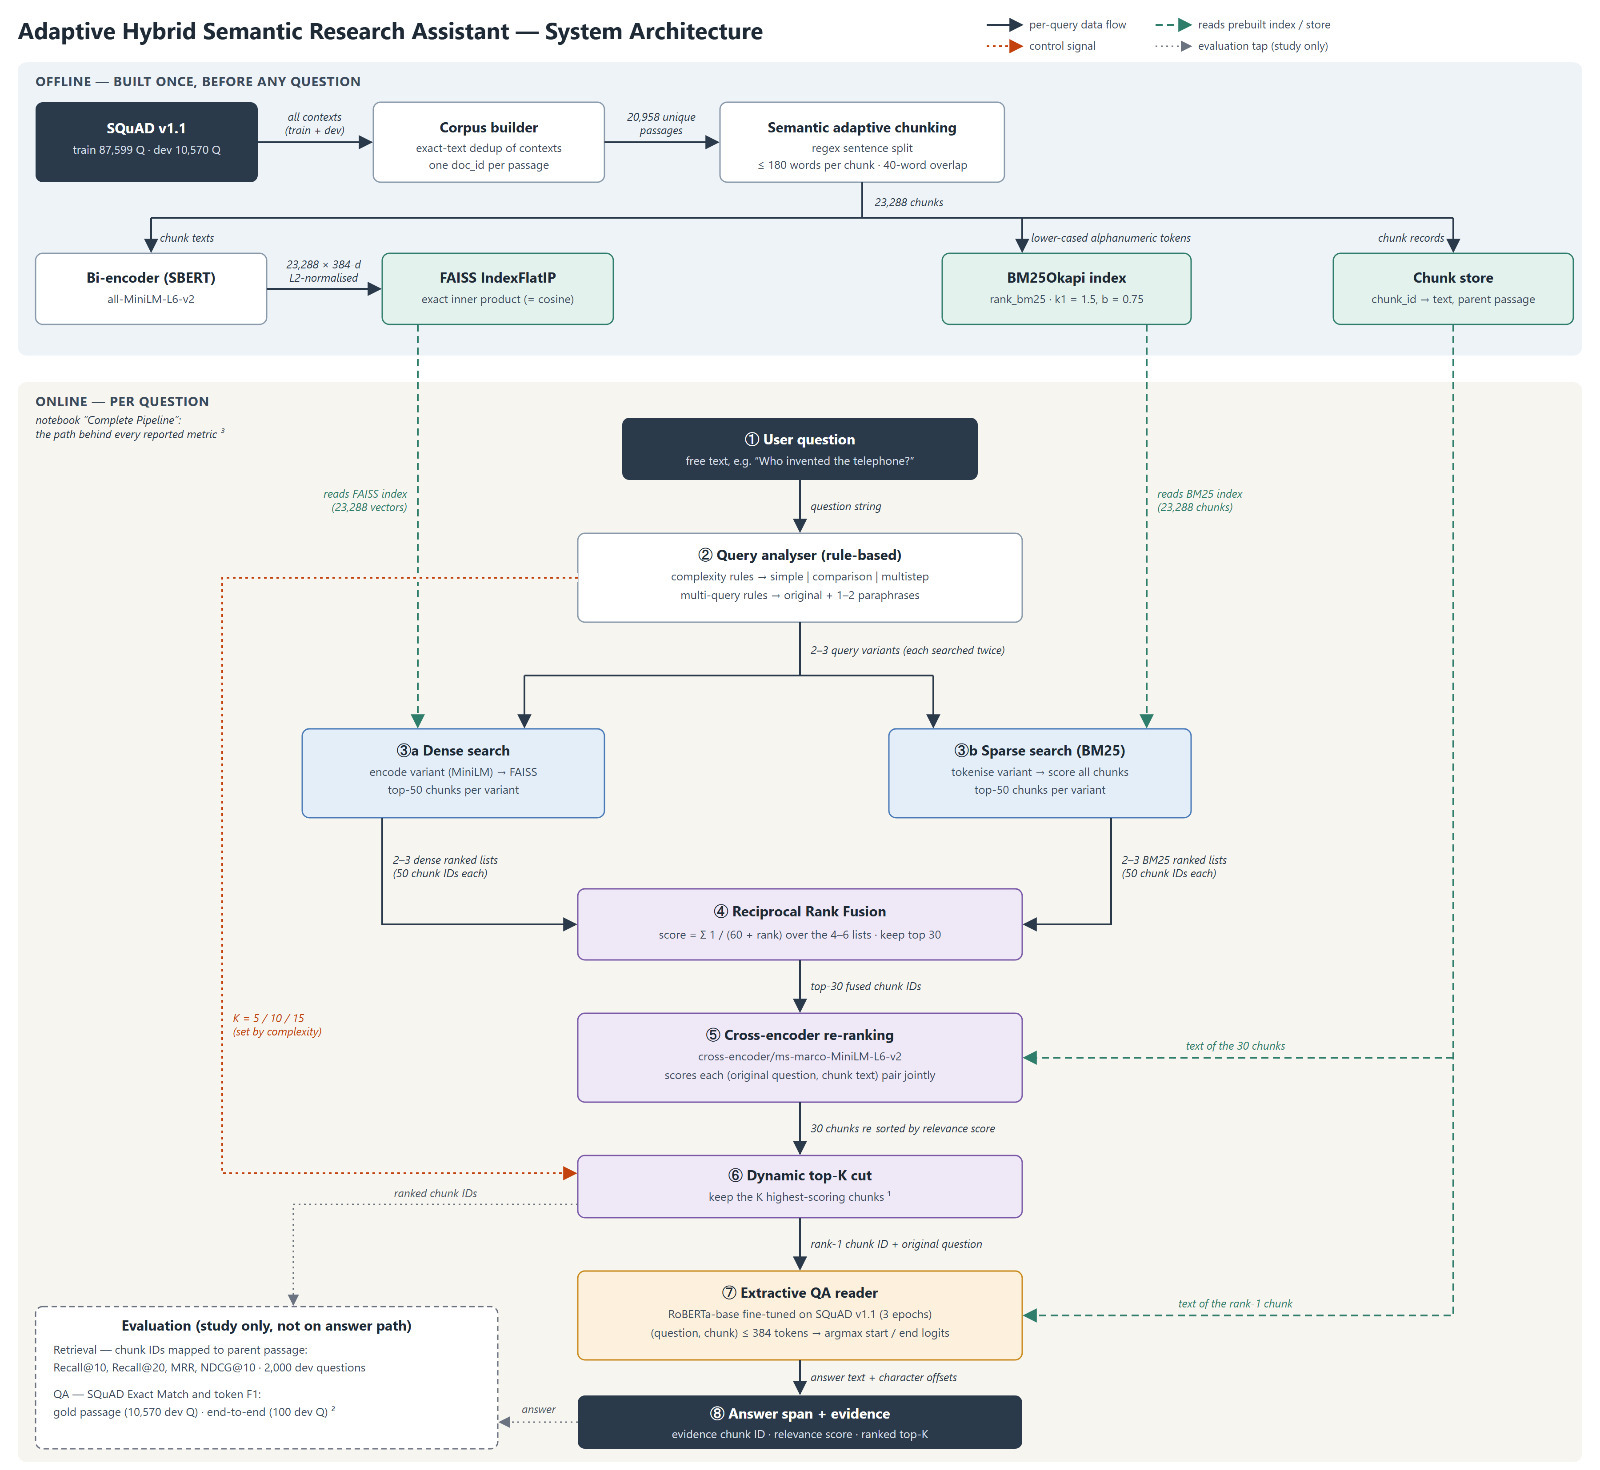
\includegraphics[width=0.97\textwidth]{figures/architecture.png}
\caption{System architecture. The offline pipeline (top) builds the dense index, the BM25 index
and the chunk store. The online pipeline (bottom) analyses the question, searches both indexes
for every query variant, fuses and re-ranks the candidates, and extracts the answer span from the
top-ranked chunk.}
\label{fig:arch}
\end{figure*}

\subsection{Corpus Construction and Adaptive Chunking}
All contexts of the SQuAD v1.1 training and development sets are de-duplicated by exact text,
giving 20,958 unique passages. Because the dense encoder truncates input beyond 256 word pieces,
each passage is split at sentence boundaries into chunks of at most 180 words, and the trailing
sentences of a chunk (about 40 words) are repeated at the start of the next so that an answer
near a boundary stays intact. This yields 23,288 chunks; the longest passage (653 words) becomes
five chunks. Every chunk keeps a pointer to its parent passage.

\subsection{Sparse Retrieval}
Chunks are lower-cased and tokenised into alphanumeric terms and indexed with BM25
\cite{robertson2009}:
\begin{equation}
\mathrm{BM25}(q,d)=\sum_{t\in q}\mathrm{IDF}(t)\,
\frac{f(t,d)\,(k_1+1)}{f(t,d)+k_1\!\left(1-b+b\,\frac{|d|}{\mathrm{avgdl}}\right)}
\end{equation}
with $k_1=1.5$ and $b=0.75$, where $f(t,d)$ is the frequency of term $t$ in chunk $d$.

\subsection{Dense Retrieval}
Each chunk is encoded with the \texttt{all-MiniLM-L6-v2} Sentence-BERT model
\cite{reimers2019} into a 384-dimensional vector. Vectors are L2-normalised and stored in a
FAISS \texttt{IndexFlatIP} index \cite{johnson2021}, so the inner product equals cosine
similarity,
\begin{equation}
s(q,d)=\mathbf{e}_q^{\top}\mathbf{e}_d,\qquad \|\mathbf{e}_q\|_2=\|\mathbf{e}_d\|_2=1,
\end{equation}
and the search is exact.

\subsection{Adaptive Query Analysis}
A rule-based analyser does two things without any additional model. First, it classifies the
question as \emph{simple}, \emph{comparison} or \emph{multistep} from cue words and punctuation
and sets the retrieval depth to $K=5$, $10$ or $15$. Second, it writes one or two paraphrase
variants of the question, so that two to three query strings are searched. Table~\ref{tab:rules}
gives the rules. For example, ``What is the speed of light?'' is classified as simple and
expanded to ``the speed of light definition?'' and ``Regarding what is the speed of light?''.
The variants change the lexical framing seen by BM25 and the embedding seen by the dense
encoder, while the cross-encoder later scores every candidate against the original question
only, so a weak variant cannot distort the final order.

\begin{table}[t]
\centering
\caption{Rules of the adaptive query analyser}
\label{tab:rules}
\footnotesize
\begin{tabular}{@{}p{0.2\columnwidth}p{0.6\columnwidth}c@{}}
\toprule
\textbf{Class} & \textbf{Trigger} & $K$ \\
\midrule
Multistep & contains \emph{and then, after, before, because, why did, how did, led to}, or at least two commas & 15 \\
Comparison & contains the word \emph{compare, versus, vs, difference, better, than} or \emph{both} & 10 \\
Simple & otherwise & 5 \\
\midrule
\textbf{Variant} & \textbf{Rule} & \\
\midrule
Definition & ``What is $X$?'' $\rightarrow$ ``$X$ definition?'' & \\
Person & ``Who \ldots'' $\rightarrow$ ``Which person \ldots'' & \\
Topic & prefix ``Regarding'' to the question & \\
\bottomrule
\end{tabular}
\end{table}

\subsection{Reciprocal Rank Fusion}
Every variant is searched in both indexes with 50 candidates each, giving four to six ranked
lists. They are fused by position \cite{cormack2009}:
\begin{equation}
\mathrm{RRF}(d)=\sum_{r\in\mathcal{R}}\frac{1}{k+\mathrm{rank}_r(d)},\qquad k=60 .
\end{equation}
A chunk that several lists rank reasonably high rises above a chunk that only one list ranks
first, and no score calibration or weight tuning is needed.

\subsection{Cross-Encoder Re-ranking}
The 30 best fused chunks are re-scored by \texttt{cross-encoder/ms-marco-MiniLM-L6-v2}, which
reads the original question and each chunk jointly. Restricting the cross-encoder to 30
candidates bounds its cost while letting it correct the order produced by the first stage
\cite{hambarde2023}. The $K$ highest-scoring chunks are returned.

\subsection{Extractive Reader}
The reader receives the question and the top-ranked chunk in one sequence of at most 384 tokens
and outputs start and end logits $\mathbf{s},\mathbf{e}$ over the tokens. It is trained with the
sum of the two cross-entropy losses,
\begin{equation}
\mathcal{L}=-\log\mathrm{softmax}(\mathbf{s})_{s^\ast}-\log\mathrm{softmax}(\mathbf{e})_{e^\ast},
\end{equation}
where $s^\ast$ and $e^\ast$ are the gold positions. Three backbones are fine-tuned: RoBERTa-base
\cite{liu2019} (primary, 125M parameters), BERT-base-uncased \cite{devlin2019} (110M) and
DistilBERT-base-uncased \cite{sanh2019} (66M). The system returns the answer span with its
character offsets, the evidence chunk, the relevance score, the softmax confidence of the
predicted start and end, and the latency.

\subsection{Implementation and Serving}
The pipeline is implemented in Python with Hugging Face Transformers, Sentence-Transformers,
FAISS and \texttt{rank\_bm25}. Both indexes are built in memory at start-up; the exact
inner-product index needs about 36~MB for 23,288 vectors of 384 dimensions. A FastAPI service
exposes the pipeline and returns, for each question, the answer span, its character offsets in
the evidence, the evidence identifier and score, the three best candidates, the detected
complexity class, the generated variants, the start and end confidences and the reader latency.
A web dashboard presents the results and lets a user switch between the three readers for the
same question.

%% ---------------------------------------------------------------------------
\section{Experimental Setup}

\subsection{Dataset}
SQuAD v1.1 \cite{rajpurkar2016} provides 87,599 training questions over 18,891 passages from
442 articles, and 10,570 development questions over 2,067 passages from 48 articles. Passages
average 117 words. The retrieval corpus is the union of both splits (20,958 passages).

\subsection{Metrics}
Retrieval is scored on 2,000 development questions, where the relevant item is the passage the
question was written for and retrieved chunks are mapped to their parent passage. For a
question set $Q$ with gold passage $g_q$ and ranked list $\pi_q$ we report
\begin{align}
\mathrm{Recall@}K &= \frac{1}{|Q|}\sum_{q\in Q}\mathbf{1}\!\left[g_q\in\pi_q^{(1:K)}\right],\\
\mathrm{MRR} &= \frac{1}{|Q|}\sum_{q\in Q}\frac{1}{\mathrm{rank}_q(g_q)},\\
\mathrm{NDCG@}K &= \frac{1}{|Q|}\sum_{q\in Q}\frac{\mathrm{DCG}_q@K}{\mathrm{IDCG}_q@K},
\end{align}
where $\mathrm{DCG@}K=\sum_{i=1}^{K}\mathrm{rel}_i/\log_2(i+1)$, with $K\in\{10,20\}$ for recall
and $K=10$ for NDCG. Recall@$K$ bounds what any reader can
achieve, while MRR and NDCG reward placing the gold passage early, which matters because the
reader consumes the top-ranked chunk. Reading is scored with the official SQuAD Exact Match (EM) and token-level F1, taking the maximum
over the reference answers of each question:
\begin{equation}
\mathrm{F1}=\frac{2PR}{P+R},\quad P=\frac{|\hat a\cap a^\ast|}{|\hat a|},\quad
R=\frac{|\hat a\cap a^\ast|}{|a^\ast|},
\end{equation}
where $\hat a$ and $a^\ast$ are the token multisets of the normalised prediction and reference.
Readers are evaluated in two settings: with the gold passage, which isolates reading quality,
and end to end, where the complete retrieval pipeline supplies the passage.

\subsection{Training Configuration}
Table~\ref{tab:hparams} lists the configuration. Each reader is fine-tuned for three epochs on
the full training set with mixed precision on one NVIDIA GeForce RTX~5060 Laptop GPU (8~GB),
using PyTorch~2.12 with CUDA~12.8. Long passages are handled with a sliding window of 384 tokens
and stride 128.

\begin{table}[t]
\centering
\caption{Configuration}
\label{tab:hparams}
\footnotesize
\begin{tabular}{@{}ll@{}}
\toprule
\textbf{Setting} & \textbf{Value} \\
\midrule
Chunk size / overlap & 180 / 40 words \\
Dense encoder & all-MiniLM-L6-v2 (384-d) \\
Candidates per list & 50 \\
RRF constant $k$ & 60 \\
Re-ranked candidates & 30 \\
Dynamic top-$K$ & 5 / 10 / 15 \\
\midrule
Max sequence / stride & 384 / 128 tokens \\
Epochs & 3 \\
Batch size & 16 $\times$ 2 accumulation (effective 32) \\
Learning rate & 1.5e-5 (RoBERTa), 3e-5 (BERT), \\
 & 5e-5 (DistilBERT) \\
Schedule & linear, 6\% warm-up \\
Weight decay / clipping & 0.01 / 1.0 \\
Precision & FP16 \\
\bottomrule
\end{tabular}
\end{table}

%% ---------------------------------------------------------------------------
\section{Results}

\subsection{Retrieval Ablation}
Table~\ref{tab:retrieval} and Fig.~\ref{fig:ablation} report the seven configurations. BM25 and
dense retrieval are individually close (86.15\% and 86.00\% Recall@10), yet their fusion reaches
91.50\%, which confirms that the two make different mistakes. Adding the cross-encoder gives the
largest single gain: Recall@10 rises to 96.25\% and MRR from 71.70\% to 85.25\%, a gain of 13.55
points. Multi-query fusion with re-ranking reaches the best Recall@20 (96.70\%).

\begin{table}[t]
\centering
\caption{Retrieval ablation on 2,000 SQuAD development questions (\%). S: sparse, D: dense,
CE: cross-encoder, Ch: chunking, MQ: multi-query}
\label{tab:retrieval}
\footnotesize
\setlength{\tabcolsep}{2.6pt}
\begin{tabular}{@{}lccccccccc@{}}
\toprule
\textbf{Configuration} & S & D & CE & Ch & MQ & \textbf{R@10} & \textbf{R@20} & \textbf{MRR} & \textbf{NDCG} \\
\midrule
BM25 only          & \cm &     &     &     &     & 86.15 & 89.60 & 69.49 & 73.39 \\
Dense only         &     & \cm &     &     &     & 86.00 & 90.55 & 63.83 & 68.97 \\
Hybrid (RRF)       & \cm & \cm &     &     &     & 91.50 & 94.60 & 71.70 & 76.37 \\
+ Re-ranking       & \cm & \cm & \cm &     &     & \best{96.25} & 96.65 & \best{85.25} & \best{87.97} \\
+ Adaptive chunking& \cm & \cm &     & \cm &     & 91.35 & 94.40 & 71.56 & 75.64 \\
+ Multi-query      & \cm & \cm & \cm &     & \cm & \best{96.25} & \best{96.70} & 85.19 & 87.91 \\
Complete pipeline  & \cm & \cm & \cm & \cm & \cm & 95.95 & 96.45 & 85.20 & 87.31 \\
\bottomrule
\end{tabular}
\end{table}

\begin{figure*}[t]
\centering
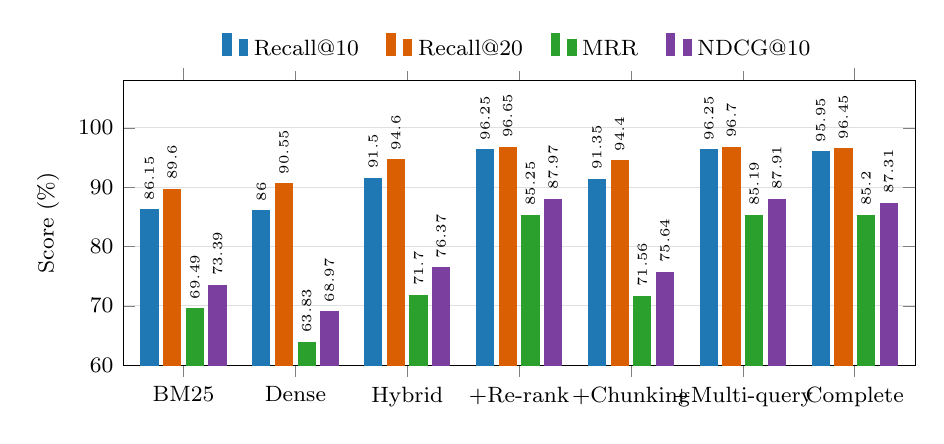
\begin{tikzpicture}
\begin{axis}[
  ybar, bar width=6.2pt, width=0.96\textwidth, height=5.2cm,
  ymin=60, ymax=108, ytick={60,70,80,90,100}, ylabel={Score (\%)}, ymajorgrids, grid style={gray!25},
  symbolic x coords={BM25,Dense,Hybrid,+Re-rank,+Chunking,+Multi-query,Complete},
  xtick=data, enlarge x limits=0.09,
  tick label style={font=\footnotesize}, label style={font=\footnotesize},
  legend style={font=\footnotesize, at={(0.5,1.03)}, anchor=south, legend columns=4, draw=none,
                /tikz/every even column/.append style={column sep=8pt}},
  nodes near coords, every node near coord/.append style={font=\tiny, rotate=90, anchor=west},
  nodes near coords align={vertical},
]
\addplot[fill=cA, draw=cA] coordinates {(BM25,86.15) (Dense,86.00) (Hybrid,91.50) (+Re-rank,96.25) (+Chunking,91.35) (+Multi-query,96.25) (Complete,95.95)};
\addplot[fill=cB, draw=cB] coordinates {(BM25,89.60) (Dense,90.55) (Hybrid,94.60) (+Re-rank,96.65) (+Chunking,94.40) (+Multi-query,96.70) (Complete,96.45)};
\addplot[fill=cC, draw=cC] coordinates {(BM25,69.49) (Dense,63.83) (Hybrid,71.70) (+Re-rank,85.25) (+Chunking,71.56) (+Multi-query,85.19) (Complete,85.20)};
\addplot[fill=cD, draw=cD] coordinates {(BM25,73.39) (Dense,68.97) (Hybrid,76.37) (+Re-rank,87.97) (+Chunking,75.64) (+Multi-query,87.91) (Complete,87.31)};
\legend{Recall@10, Recall@20, MRR, NDCG@10}
\end{axis}
\end{tikzpicture}
\caption{Retrieval quality of the seven configurations. Fusion lifts recall; the cross-encoder
lifts the rank-sensitive metrics (MRR, NDCG@10) by more than 11 points.}
\label{fig:ablation}
\end{figure*}

In terms of errors, BM25 fails to place the gold passage in the top ten for 13.85\% of
questions. The re-ranked hybrid fails for 3.75\%, so the stack removes 73\% of the misses of the
baseline (Fig.~\ref{fig:miss}). The complete pipeline, which also returns chunk-level evidence,
keeps Recall@10 at 95.95\% and improves on BM25 by 9.80 points of Recall@10, 15.71 points of MRR
and 13.92 points of NDCG@10. Table~\ref{tab:gains} summarises the gain of each step.
The cost is modest: on the evaluation hardware, hybrid retrieval
takes about 66~ms per question and the re-ranked hybrid about 150~ms.

\begin{table}[t]
\centering
\caption{Gain contributed by each retrieval step (percentage points)}
\label{tab:gains}
\footnotesize
\begin{tabular}{@{}lccc@{}}
\toprule
\textbf{Step} & $\Delta$\textbf{R@10} & $\Delta$\textbf{MRR} & $\Delta$\textbf{NDCG@10} \\
\midrule
BM25 $\rightarrow$ Hybrid (RRF)        & +5.35 & +2.21  & +2.98 \\
Dense $\rightarrow$ Hybrid (RRF)       & +5.50 & +7.87  & +7.40 \\
Hybrid $\rightarrow$ + Re-ranking      & +4.75 & +13.55 & +11.60 \\
BM25 $\rightarrow$ Complete pipeline   & \best{+9.80} & \best{+15.71} & \best{+13.92} \\
\bottomrule
\end{tabular}
\end{table}

\begin{figure}[t]
\centering
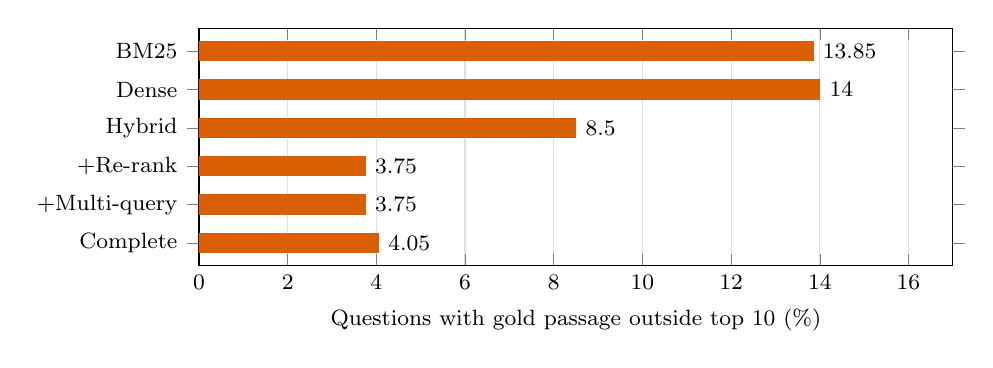
\begin{tikzpicture}
\begin{axis}[
  xbar, bar width=7pt, width=0.92\columnwidth, height=4.6cm,
  xmin=0, xmax=17, xlabel={Questions with gold passage outside top 10 (\%)},
  symbolic y coords={Complete,+Multi-query,+Re-rank,Hybrid,Dense,BM25},
  ytick=data, xmajorgrids, grid style={gray!25},
  tick label style={font=\footnotesize}, label style={font=\footnotesize},
  nodes near coords, every node near coord/.append style={font=\footnotesize},
  enlarge y limits=0.12,
]
\addplot[fill=cB, draw=cB] coordinates {(4.05,Complete) (3.75,+Multi-query) (3.75,+Re-rank) (8.50,Hybrid) (14.00,Dense) (13.85,BM25)};
\end{axis}
\end{tikzpicture}
\caption{Retrieval miss rate at rank 10. Each stage removes misses; re-ranking brings the rate
from 13.85\% to 3.75\%.}
\label{fig:miss}
\end{figure}

\subsection{Reader Comparison}
Table~\ref{tab:readers} compares the three readers. With the gold passage supplied, RoBERTa-base
reaches 85.38 EM and 91.74 F1 on all 10,570 development questions, ahead of BERT-base by 5.20 EM
and 3.89 F1 and ahead of DistilBERT by 8.40 EM and 6.22 F1. The ordering agrees with the
pre-training improvements reported for RoBERTa \cite{liu2019} and with the compression
trade-off reported for distilled models \cite{sanh2019,huang2023}.

\begin{table}[t]
\centering
\caption{Reader comparison on SQuAD v1.1. Gold: correct passage supplied (10,570 questions).
E2E: passage supplied by the complete retrieval pipeline (100 questions)}
\label{tab:readers}
\footnotesize
\setlength{\tabcolsep}{3.2pt}
\begin{tabular}{@{}lccccccc@{}}
\toprule
 & & \multicolumn{2}{c}{\textbf{Gold}} & \multicolumn{2}{c}{\textbf{E2E}} & \textbf{Latency} & \textbf{Train} \\
\cmidrule(lr){3-4}\cmidrule(lr){5-6}
\textbf{Reader} & \textbf{Params} & EM & F1 & EM & F1 & (ms) & (h) \\
\midrule
RoBERTa-base   & 125M & \best{85.38} & \best{91.74} & \best{71.00} & \best{72.34} & 8.3 & 2.45 \\
BERT-base      & 110M & 80.18 & 87.85 & 62.00 & 67.54 & 7.9 & 2.33 \\
DistilBERT     & 66M  & 76.98 & 85.52 & 60.00 & 62.41 & \best{4.3} & \best{1.18} \\
\bottomrule
\end{tabular}
\end{table}

Fig.~\ref{fig:loss} shows the training curves. All three models converge smoothly within three
epochs. RoBERTa-base attains the lowest evaluation loss (0.857 after the second epoch); the
checkpoint with the lowest evaluation loss is kept for each model. Table~\ref{tab:train} gives
the training statistics: the two 12-layer models process about 30 examples per second and
finish in under 2.5 hours, and the 6-layer DistilBERT runs at twice that rate.

\begin{table}[t]
\centering
\caption{Training statistics (3 epochs, 87,599 questions)}
\label{tab:train}
\footnotesize
\setlength{\tabcolsep}{4pt}
\begin{tabular}{@{}lccccc@{}}
\toprule
\textbf{Reader} & \textbf{Steps} & \textbf{Ex./s} & \textbf{Time (h)} & \textbf{Train loss} & \textbf{Best eval} \\
\midrule
RoBERTa-base & 8,304 & 30.1 & 2.45 & 0.938 & \best{0.857} \\
BERT-base    & 8,301 & 31.6 & 2.33 & 0.980 & 1.003 \\
DistilBERT   & 8,301 & 62.7 & 1.18 & 1.046 & 1.100 \\
\bottomrule
\end{tabular}
\end{table}

\begin{figure}[t]
\centering
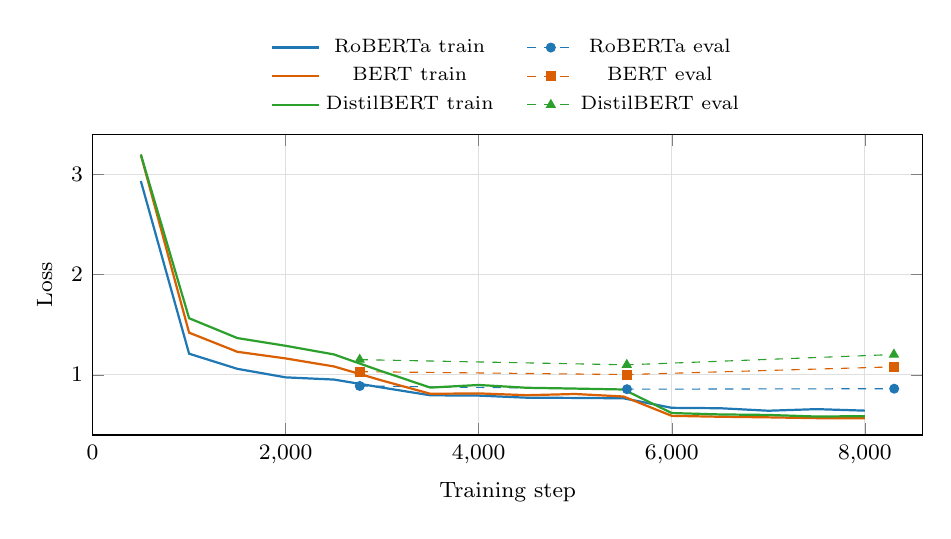
\begin{tikzpicture}
\begin{axis}[
  width=\columnwidth, height=5.4cm, xmin=0, xmax=8600, ymin=0.4, ymax=3.4,
  xlabel={Training step}, ylabel={Loss}, grid=major, grid style={gray!25},
  tick label style={font=\footnotesize}, label style={font=\footnotesize},
  scaled x ticks=false, xtick={0,2000,4000,6000,8000},
  legend style={font=\scriptsize, at={(0.5,1.03)}, anchor=south, legend columns=2, draw=none, /tikz/every even column/.append style={column sep=10pt}},
]
\addplot[cA, thick] coordinates {(500,2.934) (1000,1.211) (1500,1.060) (2000,0.975) (2500,0.953) (3000,0.873) (3500,0.796) (4000,0.793) (4500,0.772) (5000,0.770) (5500,0.766) (6000,0.671) (6500,0.667) (7000,0.642) (7500,0.658) (8000,0.643)};
\addplot[cA, dashed, mark=*, mark options={solid, scale=0.8}] coordinates {(2768,0.889) (5536,0.857) (8304,0.862)};
\addplot[cB, thick] coordinates {(500,3.196) (1000,1.421) (1500,1.230) (2000,1.164) (2500,1.084) (3000,0.943) (3500,0.811) (4000,0.815) (4500,0.797) (5000,0.809) (5500,0.784) (6000,0.591) (6500,0.582) (7000,0.576) (7500,0.568) (8000,0.567)};
\addplot[cB, dashed, mark=square*, mark options={solid, scale=0.8}] coordinates {(2767,1.032) (5534,1.003) (8301,1.080)};
\addplot[cC, thick] coordinates {(500,3.199) (1000,1.565) (1500,1.367) (2000,1.290) (2500,1.204) (3000,1.034) (3500,0.873) (4000,0.899) (4500,0.871) (5000,0.863) (5500,0.854) (6000,0.619) (6500,0.605) (7000,0.600) (7500,0.584) (8000,0.588)};
\addplot[cC, dashed, mark=triangle*, mark options={solid, scale=0.9}] coordinates {(2767,1.152) (5534,1.100) (8301,1.203)};
\legend{RoBERTa train, RoBERTa eval, BERT train, BERT eval, DistilBERT train, DistilBERT eval}
\end{axis}
\end{tikzpicture}
\caption{Training loss (solid) and per-epoch evaluation loss (dashed) of the three readers.}
\label{fig:loss}
\end{figure}

\subsection{Accuracy and Efficiency}
Fig.~\ref{fig:tradeoff} relates accuracy to cost. DistilBERT has 53\% of the parameters of
RoBERTa-base, answers in 4.3~ms instead of 8.3~ms and trains in under half the time, while
retaining 93.2\% of its F1. RoBERTa-base costs only 0.4~ms more per question than BERT-base and
gains 3.89 F1, which makes it the clear choice when accuracy matters and DistilBERT the choice
under a latency budget. All three readers answer in under 10~ms.

\begin{figure}[t]
\centering
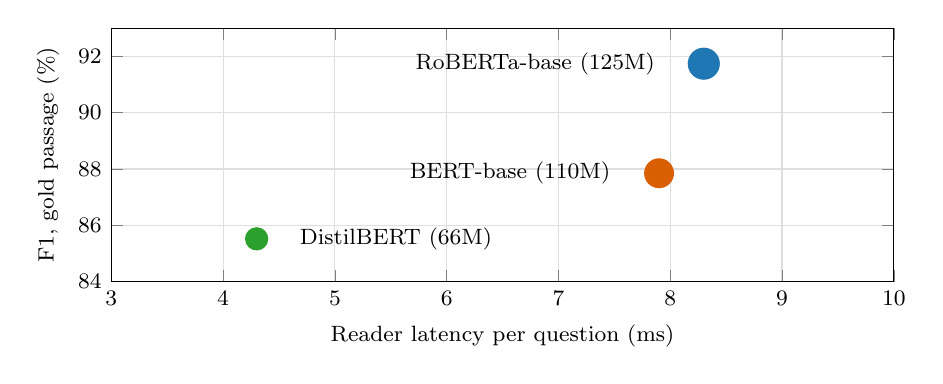
\begin{tikzpicture}
\begin{axis}[
  width=0.95\columnwidth, height=4.8cm, xmin=3, xmax=10, ymin=84, ymax=93,
  xlabel={Reader latency per question (ms)}, ylabel={F1, gold passage (\%)},
  grid=major, grid style={gray!25},
  tick label style={font=\footnotesize}, label style={font=\footnotesize},
]
\addplot[only marks, mark=*, mark size=5.6pt, cA] coordinates {(8.3,91.74)};
\addplot[only marks, mark=*, mark size=5.2pt, cB] coordinates {(7.9,87.85)};
\addplot[only marks, mark=*, mark size=4.0pt, cC] coordinates {(4.3,85.52)};
\node[font=\footnotesize, anchor=east] at (axis cs:7.95,91.74) {RoBERTa-base (125M)};
\node[font=\footnotesize, anchor=east] at (axis cs:7.55,87.85) {BERT-base (110M)};
\node[font=\footnotesize, anchor=west] at (axis cs:4.6,85.52) {DistilBERT (66M)};
\end{axis}
\end{tikzpicture}
\caption{Accuracy against reader latency. Marker size is proportional to parameter count.}
\label{fig:tradeoff}
\end{figure}

\subsection{End-to-End Evaluation}
In the end-to-end setting the reader sees only the top-ranked chunk returned by the complete
pipeline. RoBERTa-base answers 71.0\% of questions exactly (72.34 F1), retaining 83\% of its
gold-passage EM with no oracle (Fig.~\ref{fig:e2e}). Its margin over BERT-base widens
from 5.20 EM with gold passages to 9.00 EM end to end, so the stronger reader is also the more
robust one when the context is retrieved. The remaining gap between the two settings is the
retrieval-to-reader error propagation described in \cite{liu2023}; it is bounded by rank-1
accuracy, because the reader cannot extract an answer from a chunk that does not contain it.

\begin{figure}[t]
\centering
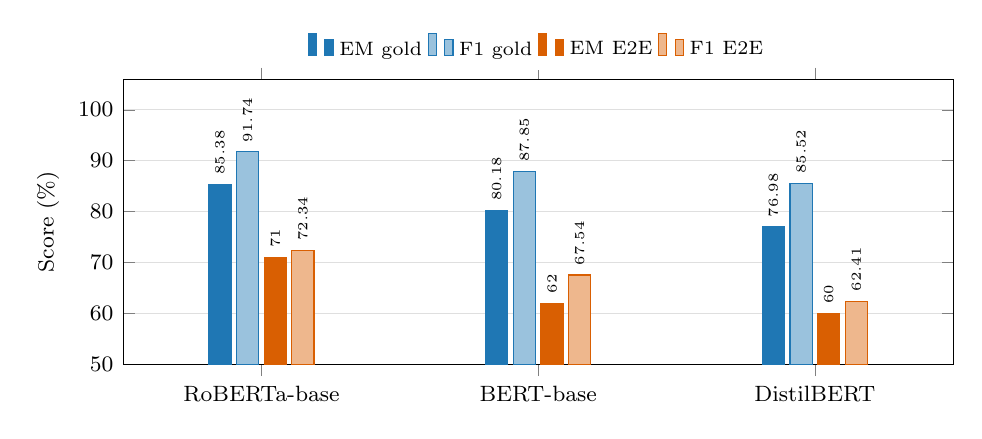
\begin{tikzpicture}
\begin{axis}[
  ybar, bar width=8pt, width=\columnwidth, height=5.2cm, ymin=50, ymax=106, ytick={50,60,70,80,90,100},
  ylabel={Score (\%)}, ymajorgrids, grid style={gray!25},
  symbolic x coords={RoBERTa-base,BERT-base,DistilBERT}, xtick=data, enlarge x limits=0.25,
  tick label style={font=\footnotesize}, label style={font=\footnotesize},
  legend style={font=\scriptsize, at={(0.5,1.03)}, anchor=south, legend columns=4, draw=none},
  nodes near coords, every node near coord/.append style={font=\tiny, rotate=90, anchor=west},
]
\addplot[fill=cA, draw=cA] coordinates {(RoBERTa-base,85.38) (BERT-base,80.18) (DistilBERT,76.98)};
\addplot[fill=cA!45, draw=cA] coordinates {(RoBERTa-base,91.74) (BERT-base,87.85) (DistilBERT,85.52)};
\addplot[fill=cB, draw=cB] coordinates {(RoBERTa-base,71.00) (BERT-base,62.00) (DistilBERT,60.00)};
\addplot[fill=cB!45, draw=cB] coordinates {(RoBERTa-base,72.34) (BERT-base,67.54) (DistilBERT,62.41)};
\legend{EM gold, F1 gold, EM E2E, F1 E2E}
\end{axis}
\end{tikzpicture}
\caption{Gold-passage and end-to-end accuracy of the three readers.}
\label{fig:e2e}
\end{figure}

\subsection{Comparison with Published Results}
Table~\ref{tab:published} sets the readers against published SQuAD v1.1 results. On the same
benchmark and metric, the RoBERTa-base reader:
\begin{itemize}
\item exceeds the original logistic-regression baseline \cite{rajpurkar2016} by 40.7 F1;
\item exceeds human performance \cite{rajpurkar2016} by 8.4 EM and 4.9 F1;
\item exceeds the published BERT-base result \cite{devlin2019} by 4.6 EM and 3.2 F1, and the
      published DistilBERT result \cite{sanh2019} by 7.7 EM and 5.9 F1;
\item exceeds the published single-model BERT-large result \cite{devlin2019} by 1.3 EM and
      0.8 F1 with about a third of the parameters;
\item is within 0.5 EM and 0.1 F1 of the BERT-large ensemble \cite{devlin2019}.
\end{itemize}
Our own BERT-base and DistilBERT readers land within 0.7 F1 of their published scores, which
confirms that the training pipeline is sound.

\begin{table}[t]
\centering
\caption{Comparison with published SQuAD v1.1 results (development set unless noted)}
\label{tab:published}
\footnotesize
\begin{tabular}{@{}lcc@{}}
\toprule
\textbf{System} & \textbf{EM} & \textbf{F1} \\
\midrule
Logistic regression \cite{rajpurkar2016}        & 40.0 & 51.0 \\
Human performance (test) \cite{rajpurkar2016}   & 77.0 & 86.8 \\
DistilBERT \cite{sanh2019}                      & 77.7 & 85.8 \\
BERT-base, single \cite{devlin2019}             & 80.8 & 88.5 \\
BERT-large, single \cite{devlin2019}            & 84.1 & 90.9 \\
BERT-large, ensemble \cite{devlin2019}          & 85.8 & 91.8 \\
\midrule
Ours: DistilBERT                                & 76.98 & 85.52 \\
Ours: BERT-base                                 & 80.18 & 87.85 \\
\textbf{Ours: RoBERTa-base}                     & \best{85.38} & \best{91.74} \\
\bottomrule
\end{tabular}
\end{table}

For orientation on the end-to-end task, Karpukhin \emph{et al.} \cite{karpukhin2020} report
open-domain EM on SQuAD questions between 20.2 and 56.5 for systems that search all of
Wikipedia, and a top-20 retrieval accuracy of 68.8\% for BM25 there. Those systems search a
corpus of about 21 million passages whereas ours searches the 20,958 SQuAD passages, so the
figures are not directly comparable; they show the regime in which our 71.0 EM and 96.70\%
Recall@20 sit. The same caution applies to the retrieval scores of \cite{mageshwari2026}
(Recall@100 83.4\%, nDCG@10 0.462), which were measured on a different collection.

\subsection{Qualitative Examples}
Table~\ref{tab:examples} lists answers returned by the deployed demonstration, which serves the
hybrid retriever with the RoBERTa-base reader. Each answer is a span of the retrieved passage and
is returned with the span confidence and the reader latency.

\begin{table}[t]
\centering
\caption{Example answers from the demonstration (RoBERTa-base reader)}
\label{tab:examples}
\footnotesize
\setlength{\tabcolsep}{3pt}
\begin{tabular}{@{}p{0.50\columnwidth}p{0.22\columnwidth}cc@{}}
\toprule
\textbf{Question} & \textbf{Answer} & \textbf{Conf.} & \textbf{ms} \\
\midrule
Which NFL team represented the AFC at Super Bowl 50? & Denver Broncos & 0.89 & 8.1 \\
In what year was Nikola Tesla born? & 1856 & 0.99 & 8.7 \\
What is Southern California often abbreviated as? & SoCal & 0.99 & 6.9 \\
When did the 1973 oil crisis begin? & October 1973 & 0.97 & 7.3 \\
What project put the first Americans into space? & Project Mercury & 0.94 & 8.1 \\
What are Ctenophora commonly known as? & comb jellies & 0.96 & 11.8 \\
\bottomrule
\end{tabular}
\end{table}

%% ---------------------------------------------------------------------------
\section{Novelty and Discussion}

The individual components are established; the novelty lies in how they are combined, adapted
and measured.

\emph{Adaptive retrieval without extra models.} Related systems adapt retrieval with learned
weights \cite{bindle2025} or with a generative model that runs for every query
\cite{mageshwari2026}. Here, complexity estimation and multi-query expansion are pure rules,
so adaptation adds only extra index look-ups.

\emph{Open and local.} The best configuration of a comparable hybrid system relies on
proprietary embeddings and a proprietary generator \cite{khan2026}. Every model here is open and
the full study, including three fine-tuning runs of 1.2 to 2.5 hours, runs on one laptop GPU.

\emph{Faithful by construction.} The answer is a span of the retrieved chunk, returned with the
chunk, its score, the character offsets and a confidence. This addresses the faithfulness risk
discussed in \cite{malin2025} structurally instead of by post-hoc checking, and complements
chunk-level grounding methods such as \cite{vake2025}.

\emph{Stage-by-stage evidence.} The ablation isolates what each stage buys: fusion adds 5.35
points of Recall@10 over BM25, and re-ranking a further 4.75 points of Recall@10 and 13.55 points
of MRR. It also reports honestly where a stage does not help on this benchmark: SQuAD passages
average 117 words, so chunking leaves recall almost unchanged, although it supplies shorter,
more focused evidence and matters more for longer documents \cite{dang2021,tan2025}.

\emph{Locating the bottleneck.} Reader comparisons usually evaluate on given passages
\cite{sinthusha2025}. Evaluating the same readers in both settings shows that the reader is
already strong and that further gains should come from rank-1 retrieval accuracy.

\emph{Deployable artefact.} The system is served through a FastAPI endpoint and a static web
dashboard that renders every reported number from the committed result files.

%% ---------------------------------------------------------------------------
\section{Limitations and Future Work}

The reader is single-hop and always returns a span, so it cannot answer questions that need
several passages or decline unanswerable ones; training on SQuAD~2.0 would address the latter.
The query variants are rule-based, and a small generative paraphraser could increase their
diversity. The bi-encoder is used off the shelf; fine-tuning it with hard negatives
\cite{choi2021,karpukhin2020} is the most direct route to higher rank-1 accuracy and therefore to
higher end-to-end accuracy. Evaluating on a larger open-domain corpus is a further step.

%% ---------------------------------------------------------------------------
\section{Conclusion}

This paper presented a retrieval-first, evidence-grounded QA system that combines sparse and
dense retrieval, rank fusion, adaptive query analysis, cross-encoder re-ranking and extractive
reading. On SQuAD v1.1 it reaches 96.25\% Recall@10 and 85.25\% MRR, removing 73\% of the
retrieval misses of BM25, and its RoBERTa-base reader reaches 85.38 EM and 91.74 F1, above human
performance and above the published BERT-base, DistilBERT and single-model BERT-large results.
End to end it answers 71.0\% of questions exactly, with evidence, confidence and latency
attached to every answer. The system achieves this with open models on a single laptop GPU,
which makes grounded, verifiable question answering practical on modest hardware.

\bibliographystyle{IEEEtran}
\bibliography{refs}

\end{document}
